%%%%%%%%%%%%%%%%%%%%%%%%%%%%%%%%%%%%%%%%%%%%%%%%%%%%%%%%%%%%%%%%%%%
\documentclass[10pt,landscape]{article}
\usepackage{amssymb,amsmath,amsthm,amsfonts}
\usepackage{multicol,multirow}
\DeclareMathOperator*{\argmax}{arg\,max}
\DeclareMathOperator*{\argmin}{arg\,min}
\usepackage{calc}
\usepackage{tikz}
\usepackage{ifthen}
\usepackage{textcomp}
\usepackage{xcolor}
\usepackage{graphicx}
\usepackage{makecell}
\graphicspath{ {./images/} }
\usepackage{enumitem}
\usepackage{bm}
\usepackage{titlesec}
\usepackage[landscape]{geometry}
\usepackage{fancyhdr}
\usepackage[colorlinks=true,citecolor=blue,linkcolor=blue]{hyperref}
%------------------------------------
\ifthenelse{\lengthtest { \paperwidth = 11in}}
    { \geometry{top=.4in,left=.5in,right=.5in,bottom=.4in} }
	{\ifthenelse{ \lengthtest{ \paperwidth = 297mm}}
		{\geometry{top=1cm,left=1cm,right=1cm,bottom=1cm} }
		{\geometry{top=1cm,left=1cm,right=1cm,bottom=1cm} }
	}
\pagestyle{fancy}
\fancyhf{}
% Remove line
\renewcommand{\headrulewidth}{0pt}
\cfoot{\fontsize{9pt}{11pt}\selectfont Frank Facundo}
\setlength{\footskip}{16pt} % amount to move footer by
% Remember to call your parents and tell them you love them!

% Define smaller plus sign
\newcommand{\plus}{\raisebox{.3\height}{\scalebox{.7}{+}}}

\makeatletter
\renewcommand{\section}{\@startsection{section}{1}{0mm}%
                                {-1ex plus -.5ex minus -.2ex}%
                                {0.5ex plus .2ex}%x
                                {\normalfont\large\bfseries}}
\renewcommand{\subsection}{\@startsection{subsection}{2}{0mm}%
                                {-1ex plus -.5ex minus -.2ex}%
                                {0.5ex plus .2ex}%
                                {\normalfont\normalsize\bfseries}}
\renewcommand{\subsubsection}{\@startsection{subsubsection}{3}{0mm}%
                                {-1ex plus -.5ex minus -.2ex}%
                                {1ex plus .2ex}%
                                {\normalfont\small\bfseries}}
\makeatother
\setcounter{secnumdepth}{0}
\setlength{\parindent}{0pt}
\setlength{\parskip}{0pt plus 0.5ex}
% ----------------------------------------------------

\title{Apache Airflow}
\begin{document}

\raggedright
\footnotesize

\begin{center}
    \vspace{-50mm}
    \Large{\vspace{-15mm}\textbf{Apache Airflow}} \\
    \footnotesize{Last Updated \today}
    \vspace{-.4mm}
\end{center}
\begin{multicols*}{3}
    \setlength{\premulticols}{1pt}
    \setlength{\postmulticols}{1pt}
    \setlength{\multicolsep}{1pt}
    \setlength{\columnsep}{2pt}
    % --------------------------------------------------------------
    \section{\underline{Airflow}}
    
    Apache Airflow is an open-source platform for developing, scheduling, and monitoring batch-oriented workflows.

    \section{\underline{Architecture}}
    
    An Airflow installation generally consists of the following components:

    \begin{itemize}[label={--},leftmargin=4mm]
        \vspace{-1mm}
        \itemsep -.4mm
        \item A scheduler, which handles both triggering scheduled workflows, and submitting Tasks to the executor to run.
        \item An executor, which handles running tasks. In the default Airflow installation, this runs everything inside the scheduler, but most production-suitable executors actually push task execution out to workers.
        \item A webserver, which presents a handy user interface to inspect, trigger and debug the behaviour of DAGs and tasks.
        \item A folder of DAG files, read by the scheduler and executor (and any workers the executor has)
        \item A metadata database, used by the scheduler, executor and webserver to store state.
    \end{itemize}


    \begin{center}
        \vspace{-1mm}
        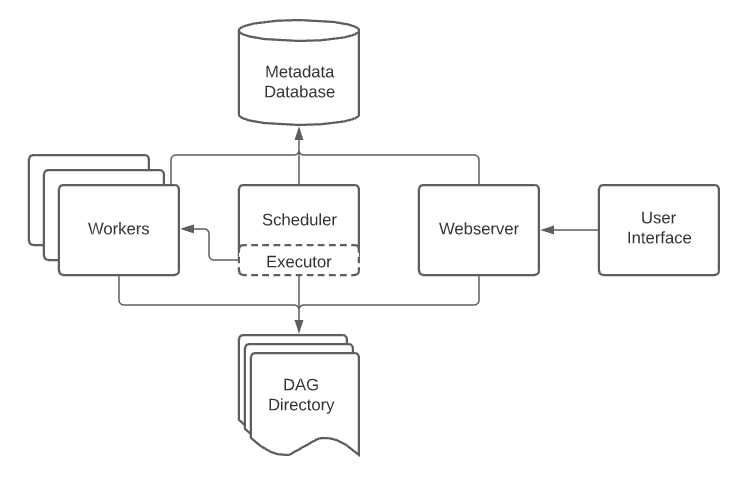
\includegraphics[scale = .4]{images/arch-diag-basic.png}
    \end{center}
    \vspace{-2mm}

    \section{\underline{Concepts}}
    \subsection{DAGs} - A DAG (Directed Acyclic Graph) is the core concept of Airflow, collecting Tasks together, organized with dependencies and relationships to say how they should run.
    Directed: Data flows only forwards and not backwards.
    Acyclic: It avoids infinite loops.
    Here’s a basic example DAG with four Tasks - A, B, C, and D:
    \begin{center}
        \vspace{-1mm}
        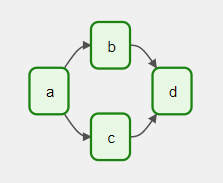
\includegraphics[scale = .4]{images/basic-dag.png}
    \end{center}
    \vspace{-2mm}

    \subsection{Tasks} - A Task is the basic unit of execution in Airflow.
    There are three basic kinds of Task: 
    \begin{itemize}[label={--},leftmargin=4mm]
        \vspace{-1mm}
        \itemsep -.4mm
        \item \textbf{Operators}: Predefined task templates that you can string together quickly to build most parts of your DAGs. 
            \subitem \textbf{BashOperator} - executes a bash command
            \subitem \textbf{PythonOperator} - calls an arbitrary Python function
        \item \textbf{Sensors}: A special subclass of Operators which are entirely about waiting for an external event to happen.
        \item \textbf{TaskFlow-decorated @task}, which is a custom Python function packaged up as a Task.

    \end{itemize}

    \section{\underline{References}}
    \href{https://airflow.apache.org/docs/apache-airflow/stable/core-concepts/overview.html}{Architecture Overview}    
    
    \href{https://airflow.apache.org/docs/apache-airflow/stable/ui.html}{UI / Screenshots}    

\end{multicols*}

\end{document}